%=======================================================================================%
% the main points of this introduction are 
% outline the complexity of biological systems for physicists
% 	> even though our theoretical models should preidct everything on the energy and length scales of biology we can't because of their heterogeneity.
%   > Give examples of the heterogenaity 
% Give some points on the history of molecular biophysics  
%   >  Hodgkin-Huxley Models
%   > Gramicidin 
% Point out how Cystic Fibrosis is an expression of this progression, going from genotype to phenotype using an ion channel to teach us biophysics. 
% conclusion.
\pagenumbering{arabic}
\chapter{Introduction: Biology, The Hardest Science}
\setcounter{page}{1}
\label{chap:intro}
\chapquote{Whatever complexity means, most people agree that biological systems have it. -Frauenfelder and Wolynes \cite{frauenfelder1994} } {}
\vspace
\section{Thesis and Chapter Summary}

This thesis seeks to apply a philosophy of molecular biophysics to demonstrate its capability to investigate pressing problems in biology and medicine. In particular, we will use molecular dynamics (MD) to look at various modes of misfunction for an anion channel, the Cystic Frosts Transmembrane conductance regulator (CFTR). These techniques will allow us to formulate a model of CFTR's misfunction which we hope will direct research efforts and allow more patients suffering from Cystic Fibrosis (CF) access life saving medication. 

In this first short chapter we will quickly build a philosophy of how to look at biology through the lens of a physicist. We will outline what the goal of a physicist is, to create abstract formalisms which can be used to model the natural world. We will then observe what makes the construction of such formalisms so dififcult in biology. We will walk through how a specific set of systems, namely ion channels have historically allowed us to take the behaviour of ion channels and climb upward to understand more complex biological systems, such as whole cells. 

In more detail, chapter \ref{chap:methods} will describe the chemical and numerical simulation techniques we have used to study the CFTR protein system, while chapter \ref{chap:cftr} gives an overview of the CFTR system itself, and also a set of \textit {in vitro} assays which compliment our computational modelling.  Chapters \ref{chap:i37r}, \ref{chap:r352q}, \ref{chap:s945l} and \ref{chap:opening} demonstrate the details of how a diverse application of the simulation techniques in chapter \ref{chap:methods} can be used to discover the unique modes of misfunction in CFTR. In combination with \textit {in vitro} cellular techniques, these simulation results prove that these mutations can be rescued by existing drug regimens. Finally, chapter \ref{chap:conclusion} ties together these results to argue for a physical model which elucidates the mechanism of action for cystic fibrosis drugs. Armed with this model we will work through the available literature and identify some priorities for future studies using molecular modelling for cystic fibrosis research.

We hope this small example can demonstrate the utility of physics expertise for the field of molecular medicine. We anticipate that such methods will only grow in power with improvements in computational and experimental techniques.

\section{What is Physics?}
When I was in high school I always described physics as ``the study of how things move". Although intuitive, this description does not shed light on the philosophy of doing physics which make it such a powerful tool for understanding the natural world. To create a predictive physical, theory one must first carefully define a naturally motivated formalism. Then, using mathematics, the implications of this formalism are built up to make predictions about measurable phenomena. Should the predictions from the formalism agree with experimental results, it validates the physical theory. This is what makes physics feel like the most "fundamental" of the sciences

These formalisms can take a few forms. Examples include:
\begin{itemize}
\item The gas of hard spheres, which we use to derive the Boltzmann's kinetic theory of gasses.  
\begin{equation}
	\label{hard_spheres}
	\frac{\partial f_1}{\partial t} + \frac{\bold{F}}{m}\cdot\nabla_\bold{r} + \bold{v} \cdot \nabla_\bold{r} f_1 =  \int \int (f'_1f'_2 - f_1 f_2) \tilde \kappa d \hat \kappa d \bold{v}_2
\end{equation}

\item The interacting electric and magnetic vector fields in Maxwell's laws of electromagnetism.
\begin{equation}
	\partial_\alpha F^{\alpha \beta} = \frac{4\pi}{c} J^\beta
\end{equation}

\item The Riemannian manifolds which define the curvature of spacetime in Einstein's theories of relativity.
\begin{equation}
	G_{\mu \nu} + \Lambda g_{\mu \nu} = \kappa T_{\mu \nu}
\end{equation}

\item The complex probability waves which evolve according to Schr\"oedinger's wave equation, describing quantum mechanics. 

\begin{equation}
	i \hbar \frac{d}{dt} | \psi (t) \rangle = \hat {H} | \psi (t) \rangle 
\end{equation}
\end{itemize}

As biophysicists we would wish to the most basic formalisms in biological phenomenon. The quest for such a formalism has an interesting origin. In 1944 Erwin Schr\"oedinger wrote an essay titled ``What is Life?" This remarkable work was written before the discovery of DNA's structure or the maturation of information theory. Schr\"oedinger uses first principals in thermodynamics and quantum mechanics to speculate at the nature of life at the atomic level. The most remarkable thing about this essay is how much the author gets right. 

He observes that since organisms exist at temperatures on the order of $10^2 $ Kelvin the phyical encoding of genetic information inside cells must be chemical in nature, as physical arrangements of atoms would be unstable at such temperatures without chemical bonds. Schr\"oedinger posits the existence of what he calls an ''aperiodic crystal". Although not a crystal in the rigorous sense, the double helix structure of DNA is not far off such an analogy. As figure \ref{dna_structure} shows, the DNA double helix is a combination of periodic and aperiodic elements, conceptually reminiscent of what one would expect of an aperiodic crystal \cite{varn2016}. This allegory is an example of how physical principals can in fact be used to direct questions in fundamental biology. In fact, James Watson credited Schro\"edinger's book as one of his influences to study genetics \cite{watson2010}.

\begin{figure}
	\begin{center}
		\includegraphics[width=1.0\textwidth]{figures/dna_backbone_aperiodic_crystal.pdf}
	\end{center}
	\captionsetup{singlelinecheck = false, justification=raggedright}
	\caption[The Structure of DNA has Periodic and Aperiodic Elements] {\textbf{The Structure of DNA has Periodic and Aperiodic Elements}}{Although not a crystal, the structure of DNA has some periodic and some aperiodic elements. This is reminiscient of Schr\"oedinger's speculation that genetic information is chemically encoded in an aperiodic crystal or an aperiodic solid. }
	\label{dna_structure}
\end{figure}

Here, Schr\"oedinger has naturally chosen the formalism of interacting atoms, consistent with the statistical mechanics in equation \ref{hard_spheres}, to arrive at his model of an aperiodic crystal. In this thesis, as chapter \ref{chap:methods} justifies, we will use a more careful, but similar formalism to study the function of the CFTR protein. The goal of chapters \ref{chap:i37r}, \ref{chap:r352q}, \ref{chap:s945l} and \ref{chap:opening} is to develop a molecular model of Cystic Fibrosis disease which we will analyse in chapter \ref{chap:conclusions}. The model we arrive at is more abstract than we are used to for physicists and the next section will explore why this is the case for biological systems
 
%Somewhere on the scale between a single protein and a single cell this is what we consider "life". We have single unicellular organisms but we don't have uniproteomic organisms. So the fundamental length scale of life is somewhere between $10^{-10}m$ and $10^{-3}m$. This is the first loop in our strange loop.

%Biological strange loops would not seem to be as self similar as the clean nice logics in the strange loop of the Godelian knot. Why is this?

\section{The Physics Inside your Cells}
%purpose of this section is to 

Why can't I write down an equation which will tell me how long I will live? Or how tall I will grow?

These might seem like odd questions but if you asked a physicist how much power it would take to ionise a gas or how long it will take a black hole to evaporate and they will have highly accurate models at the ready to answer easily. 

What makes the first set of questions so much more difficult to answer?

A physical theory such as those in the list in the previous section may fails for one of two reasons. Either we do not have sufficient computational power to integrate the formalism high enough to describe a specific phenomenon, or the formalism disagrees with experimental measurements of a phenomena. Quantitative theories of biology, from a fundamental physics point of view, fall firmly in the former category. Our current physical theories have sufficient accuracy at the energy and length scales of biology that we can accurately model every phenomenon inside a living being \cite{carroll2021}. 

 The difficulty of studying biology does not arise from complex interactions. As we will see in chapter \ref{chap:methods} the interactions between atoms within living things is surprisingly simple and a formalism of interacting atoms is appropriate for modelling cellular functions. Rather, the complexity arises from the sheer number of interactions we must consider. Inside cells we find proteins, lipids, solvents, salts each with their own properties. Biophysics distinguishes itself from more traditional physics as it considers systems that are highly heterogeneous and anisotropic. This makes it difficult to scale up formalisms using human tractable mathematical tools. The more heterogeneous the system the more complex the mathematics becomes and thus, the more we must rely on brute force computation of a lower level theory.

 That is not to say we can simply solve all biological with brute force computation. There is a rich field of biological mathematics which shows how elegant applications of mathematics can shed light on macroscopic biological systems. We will see this in the exmaples of the conduction of signals through a nerve. 

This heterogeneity is perhaps why this thesis contains passages on quantum mechanics all the way up to patient lung capacity.

%For biological systems there appears to be too much complexity for such analogies to have the same level of success. 

The heterogeneity of biology is easy to observe. If you look at your arm, you will notice hair, pores, dry skin, dead skin, perhaps even tendons and muscles twitching beneath the surface. If you were to take a single cell from just beneath the skin and stain it to distinguish features in an electron microscope, you would find all sorts of complex structures called organelles. The size, shape and function of these elements would be different if the cell was taken from somewhere else in your body. Within and between each those organelles is a salty, wet dance of molecules large and small. This journey from your arm to your organelles spans 5 orders of magnitude. The complexity across length scales hints at the reasons behind biology's physical complexity. Plasma physicists may use the same mathematical tools to describe materials as diverse as the dense stellar core to the sparse intergalactic nebulae these span 28 orders of magnitude in density \cite{chen2018}. Would that we were so lucky in biology where we struggle to apply same physical models to deal with phenomena across a single order of magnitude.  

Although considerable success can be found in modelling biology with formalisms that do not include the phenomenon of interacting atoms, they must be taylor made in order to model specific phenomenon \cite{phillips2012}. The advantage of molecular dynamics and the formalism of interacting atoms in chapter \ref{chap:methods} is that they are the most accurate available to the biophysicist. The issue is the considerable computational load attached to them. 

Thus, in order to move towards more predictive theories of biology it is necessary to develop layers of physical theories applicable in different contexts., to consider much more of the fundamental physical processes occurring within biological systems than simply searching for statistical trends. One form of this from fundamentals approach is the simulation of every atom in a biological system. Although computationally expensive, this approach has been proven necessary due to the heterogeneous nature of biological systems \cite{moy2000, corry2000a}. When it comes to small changes to proteins, we can sadly get away with very little idealisation when it comes to the molecular details of proteins.


%One of the things we're trying to do with molecular dynamics is fill in the gap left by the sequence->function paradigm which is internalised in current understandings of molecular biology. We usually talk about how the sequence of the gene defines its function because it gives the protein its structure but really there is a considerably larger amount of regulatory pressure exerted by the environment. This is what is missing from the sequence alone paradigm.

%Biological systems exhibit such a problem for the physicist because unlike the above problems it is extremely hard to pick out a fundamental unit to even begin our upwards journey. An evolutionary biologist might say to choose the "gene" but this is actually far too high in our spatial heirarchy already. Really, a gene is only meaningful to the dance of life if it has partners to dance with. 

%A coil of DNA in water doesn't really do much in solution except decay without machinery that can preserve, read, translate and replicate it. The gene is an emergent property, we have to go deeper. 

%So, what are the gene's partners? 

%A slew of biological machinery that mostly take the form of proteins. These proteins are a special case of chemistry, with many observable functions. Their sequence is  coded by the DNA in something reminiscent of a strange loop \cite{hofstadter2007}. 

%This self referential loop is one of the reasons biology is so difficult. Since we know that this strange loop is kicked off by atomic interactions we will start there. As we are taking a physical, pragmatic approach here it would make sense to begin with the protein, after all, they stave off the march of entropy constantly trying to eat up all of your cells. It also just so happens that they are much easier to understand computationally since their motions are faster and more flexible. 

%The first level sub cellular organisation is perhaps the most intimdating first step for me personally after spending 4 years simulating a single protein. Glimpsing the complexity within a single one of these molecules has been one of the most existential experiences of my life but the knowledge that there are astronomical numbers of these things inside me all of the time terrifies me.

%It is hoped that illustrating the monumental amount of both intellectual effort and material resources of incrementally increasing the understanding of a single protein amongst the 23000 or so encoded in our genome will give the reader and understanding of how we might continue our quest to understand the molecular dance that plays within all of us.

%After this things start to run away from me with my handful of GPUs and limited patience. So in this thesis we will only discuss single proteins.

\section{Using Ion Channels as Natural Laboratories to Learn Biophysics}

Ion channels are a special kind of protein which allow the passive of charged particles through a cell membrane. They are excellent laboratories for the study of biophysics for two reasons. Firstly, it is very easy to measure their activity with a technique called electrophysiology \cite{}, because we are simply measuring current. Secondly, they are critical to the health and function of cells. As cell biology has advanced it has become clear that the polarisation state (potential difference from the inside to the outside) of a cell is critical to its function. Changes to the polarisation regulate many chemical reactions inside the cell \cite{catterall2011, muthuswamy2012, levin2014, levin2014a}. 

It is perhaps then not surprising but nonetheless remarkable that ion channels are the targets of 19\% of clinically approved drugs \cite{santos2017}. However, there is much more work to be done as candidates drugs are often insufficiently selective for the clinically optimal ion channel subtypes \cite{stansfeld2006, kaczorowski2008, waszkielewicz2013}.

Historically, ion channels have served as a testing ground for biophysical models. The first breakthrough in modelling the behaviour of ion channels comes from the experiments of two biophysicists, Hodgkin and Huxley. These mathematicians took nerves from giant squid and measured the current running through the nerve in response to electrical stimulation. What they found was intriguing. Signals would only propagate down the nerve when the input signal was of a sufficient voltage. They managed to match their experimental data with a model comprised of the following set of ordinary differential equations:

\begin{equation}
	\label{hh_equations}
\begin{aligned}
	I = C_m \frac{dV}{dt} &+ \bar{g}_K n^4 (V - V_K) + \bar{g}_{Na} m^3 h (V - V_{Na} ) + \bar{g}_l (V-V_l) , \\ \\
	\frac{dn}{dt} &= \alpha_n(V)  (1-n) - \beta_n(V)  n, \\
	\frac{dm}{dt} &= \alpha_m(V)  (1-m) - \beta_m(V)  m, \\ 
	\frac{dh}{dt} &= \alpha_h(V)  (1-h) - \beta_h(V)  h  
\end{aligned}
\end{equation}

Here, the $n,\ m$ and $h \in [0,1]$ parameters are associated with potassium channel subunit activation, sodium channel subunit activation, and sodium channel subunit inactivation, respectively. $C_m$ is the capacitance of the lipid membrane per unit area, and $\bar{g}_i$ is the maximal conductance allowed across the membrane, per unit area. The terms $V_i$ denote either the total voltage or the contribution to the total from a specific charged species.

The solutions to the Hodgkin Huxley model allow us to mathematically discover and describe several important cellular functions. The model encodes the existence of a cell's resting potential and selective voltage gated ion channels. Even today, the molecular mechanisms behind these discoveries are used understand protein and cellular function \cite{}. 

This is an example of the development of a mathematical formalism n equations \ref{hh_equation} is not fundamental in the same way as equations found in physics theories but it is built for an express purpose, to model the propagation of signals through a nerve. This model shows how quantitative thinking can lead to insights in biology. The sheer complexity of biology demands this of us. We cannot create complete theories so we must find useful formalisms for small domains of the problem space.

In this thesis we aim to do something similar, by building up from fundamental physics outlined in \ref{chap:methods} we will build a model for the disfunction of a single gene (CFTR) to understand a disease (CF). Again, we do not posess sufficient computational power to produce a complete physical model of CF, so we will have to settle for a qualitiative model which we will outline in \ref{chap:conclusions}. 

%The measurements and modelling they carried out gave an exciting set of results. They found that the cell had to maintain a constant voltage gradient, they discovered that the presence of voltage gated ion channels and cation selective ion channels\cite{hodgkin1952}. Each of these features, motivated by mathematical modelling have been found to be critical to the functioning of the cell and fundamental to the foundation of molecular biophysics.    

\begin{figure}
	\begin{center}
		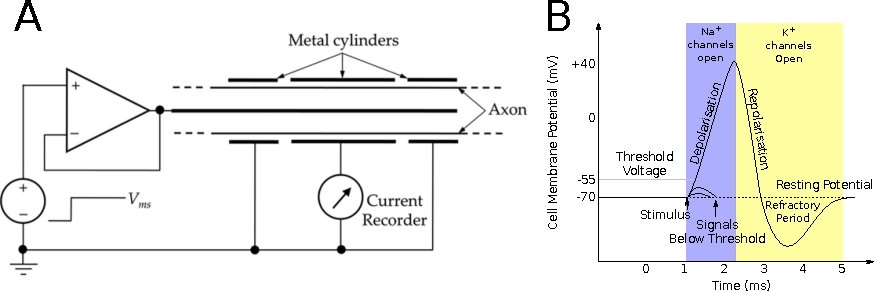
\includegraphics[width=0.5\textwidth]{figures/Hodgkin-Huxley_action_potential.pdf}
	\end{center}
	\captionsetup{singlelinecheck = false, justification=raggedright}
	\caption[The Action Potential is a Solution to the Hodkin-Huxley Model] {\textbf{The Action Potential is a Solution to the Hodgkin-Huxley Model }}{The shape of the action potential is a similar sight in many physiology textbooks. It was is in fact discovered as a result of the mathematical modelling of Hodgkin and Huxley hinting at the deep biophysics of ion channels won them the 1963 Noble Prize in medicine. This discovery is an excellent example of how deep theoretical insight can lead to predictable models of living systems \cite{hodgkin1952, hodgkin1952a, hodgkin1952b, hodgkin1952c, hodgkin1952d}.}
	\label{action_potential_graphic}
\end{figure}

In addition to the mesoscopic models ion channels spawned by hodgkin and huxley, there has been considerable interest in these systems from  the early adopters of computational molecular biophysics. Biophysicists such as Martin Karplus, Beno\^it Roux, Shin Ho-Chung, Mark Sanson, Serdar Kuyucak and Toby Allen have devoted significant parts of their career to studying ion channels\cite{sansom1991, roux1991, sansom1991, allen2003, allen2004, chung2002, tieleman2001}. 

Early studies usually focussed on gramicidin A (gA) as a toy model for the diffusion of charged species. With the advances of this kind of modelling and experimetnal techniques the molecular details of the function of ion channels has become accessible to computational techniques. 

The work on gA enabled careful studies of potassium channels \cite{rashid2013, li2021, flood2021}. Quite rapidly, the availability of protein structures and the maturation of these computational methods has enabled diverse studies of ion channels and other ion channel protein systems \cite{lev2020, chen2021}.


\begin{figure}
	\begin{center}
		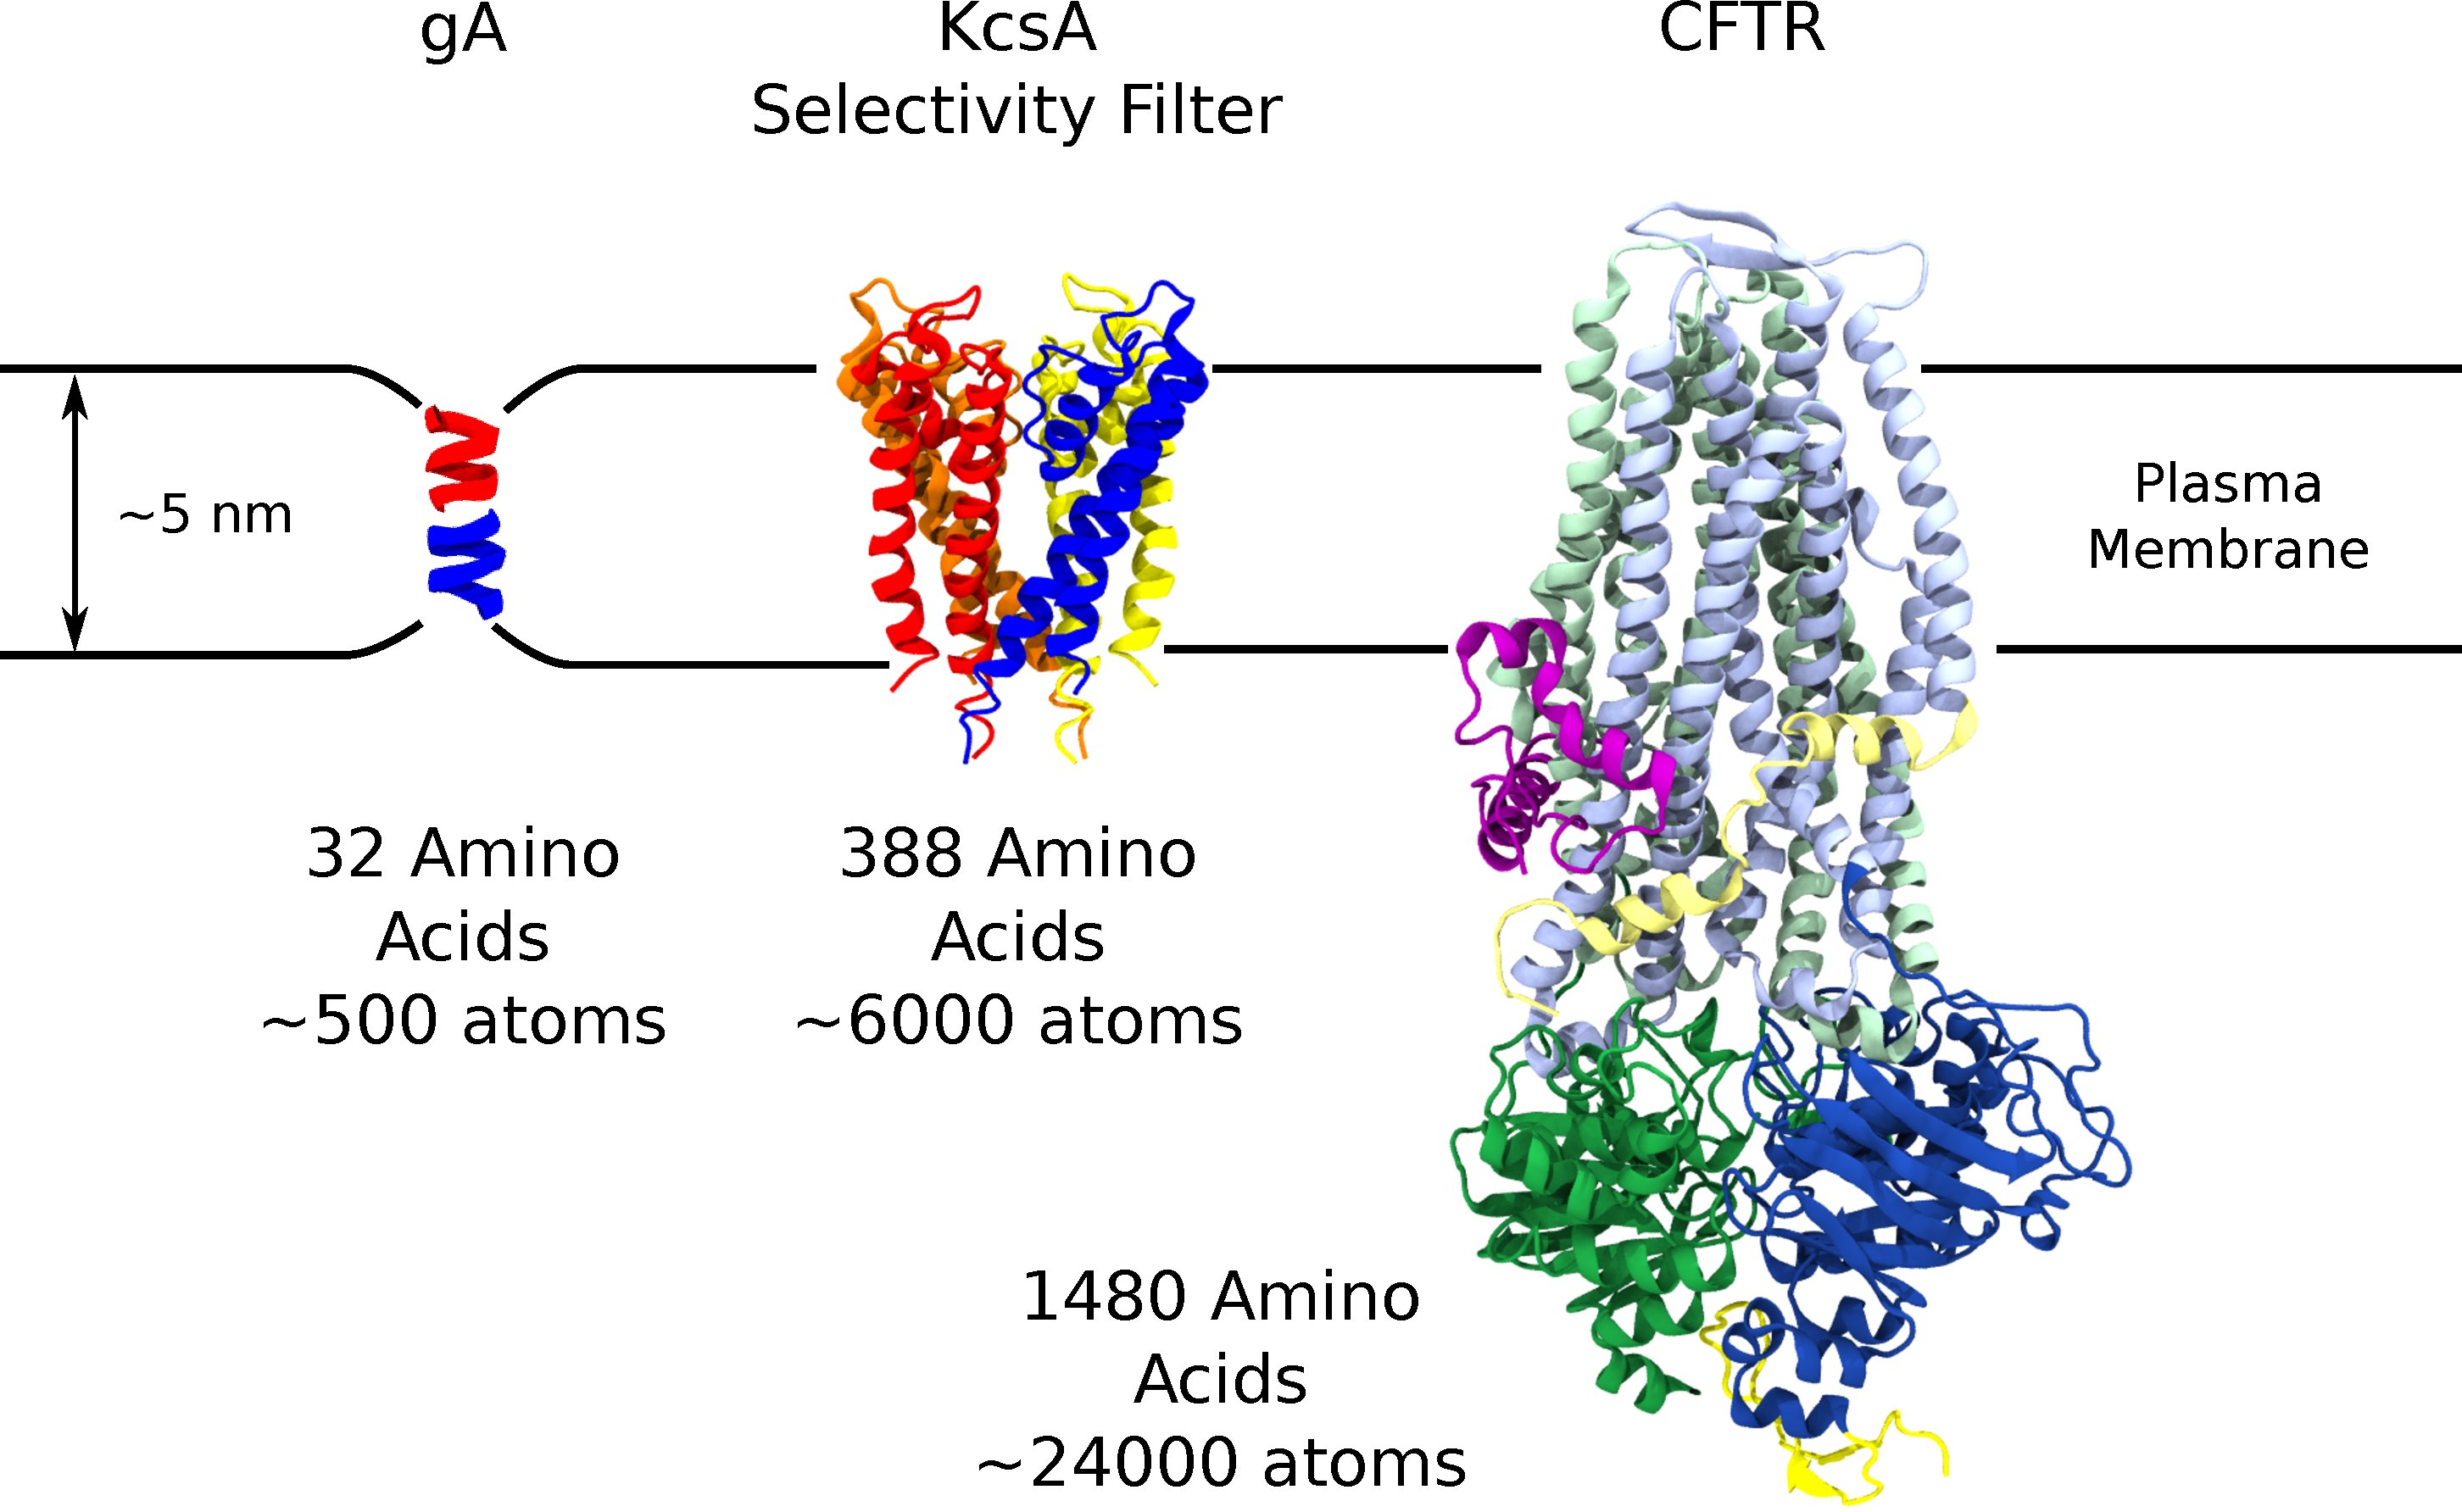
\includegraphics[width=0.8\textwidth]{figures/ion_channel_progression.pdf}
	\end{center}
	\captionsetup{singlelinecheck = false, justification=raggedright}
	\caption[Some ion channels] {\textbf{Some ion channels}}{Three ion channels which reflect the progress of molecular modelling. Gramicidin A has historically been used as a toy model to test different modelling techniques (PDB ID 1NT5) \cite{sham2003}. KcsA is a bacterial potassium channel which . This structure only comprises the pore domain, sometimes called the selectivity filter (PDB ID 1BL8) \cite{doyle1998}. Finally, the CFTR anion channel which this thesis is written about (PDB ID 6MSM) \cite{zhang2018a}. Interestingly, each of these structures was solved with a different structural biology method. Solid state Nuclear Magnetic Resonance imaging, X-Ray Crystallography and Cryogenic Electron Microscopy respectively.}
	\label{action_potential_graphic}
\end{figure}

Until recently, there have been a limited number of structural targets for biophysicists to work with. Initially, inquiries were limited to modelling gramicidin A, an antibacterial peptide which assembles into an ion channel in the cell walls of gram positive bacteria\cite{liou2015}. The mechanism of action for this little peptide is to simply destroy the bacterium's ability to hold an ion gradient. This causes the cell to dis regulate in all sorts of ways, such as the inability to produce ATP.

Gramicidin is one of the toy systems we use as biophysicists to develop theoretical methods. The others being the dialanine peptide, decalanine and sometimes ubiquitin \cite{}.

The discovery of voltage gated channels and a resting potential are still subjects studied in cell biology today as they are critical to the cells' function \cite{}.

These factors have to allowed biophysicists sufficient data to build sufficiently accurate models of protein systems which generalise. Leading to a thriving field, analysing systems as diverse as photocells to gold nano particles CITATIONS NEEDED. \ref{chap:methods}

So by using ion channels as basic biophysical laboratories have been used consistently to understand higher level protein physics \cite{}, and now we can apply this molecular understanding to attempt to tackle other diseases as experimental techniques have improved such as diabetes, and neurodegenerative diseases \cite{}. Building an atomistic understanding is allowing us to study medicine with atomic precision.

%=======================================================================================%

\section{Studying Cystic Fibrosis, Toward a Molecular Theory of Disease.} 

The sad truth of CF is that those afflicted are extremely unlucky. A single, change to the genome and their lungs fill with sticky mucus and become infected with bacteria, each breath cumbersome. Personally, I've not met somebody who has this disease. I have consistently wondered what perspective I'm missing by not suffering myself from such a condition or even knowing somebody with it. I'm not been trained in the ethics of studying medicine.

In this way, my motivations for studying the CFTR protein aren't solely focussed on treating disease. There is a perspective on protein evolution which states that the primary sequence of a particular gene contributes to the overall fitness of an organisms by a formula \cite{depristo2005a}.

\begin{equation}
	W(\Delta G) \propto \exp\bigg(\bigg[-\frac{\Delta G - \Delta G_{opt}}{\sigma_{\Delta G}}\bigg]^4\bigg) + c
\end{equation}

Where $W$ represents the fitness of the organism, $\Delta G$ is the folding energy of the protein and $\Delta G_{opt}$ is the folding energy of the protein . Figure \ref{fitness_landscape_gene_figure} demonstrates the types of random walks of a gene through sequence space which this model predicts. 

It just so happens that the CFTR gene sits at the precipice of a daunting cliff in sequence space. Where the band of stability in the modified gaussian in figure \ref{fitness_landscape_gene_figure} is extremely narrow. So by taking small steps in sequence space and plunging down this cliff we can try to understand how we might push the ball back up the cliff and retain functionality.

Moreover, by learning the nuts and bolts of what goes wrong with CFTR we can start to think about where some of these cliffs might be in other places in the proteome, to gain function and avoid disease and debilitation.

The reality of disease pathogenesis being caused by so many different mutations means that there has been decades of investigation into the function of every domain in the protein. 

This theoretical model is informs the conclusions of chapter \ref{chap:conclusions}.

Due to the array of disease causing mutations which occur across the cystic fibrosis protein, there is a large body of literature on its unique function. This allows us a glance into its function and an opportunity to simultaneously perform basic biophysical research while directly assisting in furthering patient outcomes. This is the sort of inquiry which drives basic science forward, combining interesting experimental data into theoretical models to make testable predictions. The aim of this thesis is to build a model to make predictions about which kind of drugs will produce positive patient outcomes.

As we will see in chapter \ref{chap:cftr} the integration of basic biology into the treatment of cystic fibrosis has drastically improved patient outcomes. The opportunity of this thesis to shed light on the molecular details of this disease could lead to much greater patient outcomes. 

\section{The Future is Biological}
We are on the cusp of developing biology from a descriptive to a predictive science \cite{kochanski1973,liu2005, mogilner2016, covert2021, jumper2021}. This transition is driven by the refinement of experimental techniques, strong theories and powerful computational engines to link the two. As an example of what will soon be possible.

Throughout science, the integration of experimental data with theoretical models leads to new and exciting research, this is particularly true in biology with its important applications in medicine, agriculture and increasingly, manufacturing. Wet lab biologists take advantage of experimental techniques which allow them to understand the dynamics and structure of living things from the top down. The finer the experimental instrument, the finer the detail they may resolve. Conversely, computational and theoretical biologists take a bottom up approach, we aim to take the granular details of a system, and integrate them upwards to model the macroscopic behaviour of that system. With more powerful computers and more detailed models we can make predictions about the behaviour of more complex systems. What is so exciting about the current era of biological research is that the domains of these two approaches are beginning to overlap, where they can synergize  and drive further breakthroughs. As we discover more systems where this overlap can be found we will develop more sophisticated treatments for diseases and problems found around the world.

The reason this has happened before in physics is two fold. Physical systems are much more homogeneous. So it's much easier to integrate upwards in length scale. Once you understand the pairwise interaction between two components it's simply a question of having the theoretical and computational capacity to model the bulk behaviour of that system. 

The difference with biological systems is that they have so many different components that finding an analytic or even computationally tractable solution is usually impossible. However, as we collect more data and build more powerful computers we can approach more complete models. These in turn inform more powerful theoretical models these help direct the material efforts of experimental expertise . 

While previously we were limited it functional data concerning ion channels we now have unprecedented resolution for the structure dynamics for the inside of a cell. Advances in cryogenic electron microscopy, confocal microscopy, X-ray Crystallography, fluorescent microscopy and genetic engineering allow us to glimpse unprecendented information about the salty dance of life inside cells.

Alphafold is a good example. This new breakthrough builds on decades of inquiry from the structural biology community and advancements in AI to give high resolution protein structures. Now this result can be used to fill in the gaps of structural biology. Crucually, alphafold konws what it doesn't know. So we can tell where to direct the efforts of structural biology. Together these advances will fill more gaps in our knowledge of protein physics. 

Armed with this philosophy we will delineate how to use the formal object of the Schr\"oedinger wave equation to make approximations to atomic systems in order to create a biophysical model for macromolecular systmes like proteins.
